\documentclass[12pt,a4paper]{article}
\usepackage[english]{babel}
\usepackage[margin=2.5cm]{geometry} %Global margins :)
\usepackage{graphicx}
\usepackage{nicefrac}
\usepackage[modulo]{lineno}
\usepackage{amsmath}
\usepackage{amssymb}
\usepackage{multirow}
\usepackage{units}
\usepackage[section]{placeins}  %prevent floats from being moved over section headings
\usepackage{amsbsy}  % enable bold greek letters in math mode
\usepackage{booktabs}
\usepackage{authblk}   % manage author/affiliations

\bibliographystyle{plain}

% \textheight 24.0cm
% \topmargin -1cm
% \addtolength{\oddsidemargin}{-.5in}
% \addtolength{\evensidemargin}{-.5in}
% \addtolength{\textwidth}{1in}
%  \parskip 7.2pt

\newcommand{\eV}{\, \mathrm{eV}}

\usepackage{color}
\usepackage[]{hyperref}
\hypersetup{
    pdftitle={SD1500 Efficiency},
    pdfauthor={Brichetto Orquera},  
    bookmarksnumbered=true,     
    bookmarksopen=true,         
    bookmarksopenlevel=2,       
%    colorlinks=true,            
    pdfstartview=Fit,           
    pdfpagemode=UseOutlines,    
    pdfpagelayout=TwoPageRight
}

\usepackage{fancyhdr} %Header with the nice line in the top

\pagestyle{fancy}
\fancyhead[R]{GAP Note XX-YY}
% \fancyhead[L]{P. Gabriel Brichetto O.}
% \fancyfoot[C]{\leftmark}
% \fancyfoot[R]{\thepage}

\renewcommand{\headrulewidth}{1pt}


%%%%%%%%%%%%%%%%%%%%%%%%%%%%%%%%%%%%% Body %%%%%%%%%%%%%%%%%%%%%%%%%%%%%%%%%%%%%


\begin{document}

%TODO Include GAP number before submitting

\title{\textbf{Measurement of the efficiency of the 1500-metre surface detector with the 750-metre detector}}



\author{Gabriel Brichetto Orquera}
\author{Diego Ravignani}
\affil{\scriptsize ITeDA (CNEA, CONICET, UNSAM), Buenos Aires, Argentina}

\date{\vspace{-2cm}} %removes the date :)

\maketitle

% \begin{abstract}
% \end{abstract}

%%%%%%%%%%%%%%%%%%%%%%%%%%%%%% Introduction %%%%%%%%%%%%%%%%%%%%%%%%%%%%%%%%%%%%

\section{Introduction}





$E_0(\theta)=p_0+p_1\sin^2(\theta)+p_2\sin^4(\theta)$, $b=const.$ $b(\theta)=b_0+b_1\sin^2(\theta)$
%%%%%%%%%%%%%%%%%%%%%%%%%%%%%%% Efficiency %%%%%%%%%%%%%%%%%%%%%%%%%%%%%%%%%%%%%

\section{Efficiency of the 1500-metre array}
\label{sec:efficiency}

Since the SD750 is nested within the SD1500, we used the SD750 dataset as a reference and we looked for how many of these events were detected simultaneously by the SD1500. The time period used was between the incorporation of ToTd and MoPS triggers, Jan 1st 2014 to just before the AMIGA comm crisis, Aug 31st 2018, in order to get fully comparable results between the datasets including only the original triggers and the new triggers and to avoid the T3 error rate spike.

For the energy estimator of the SD1500 events we proposed the energy of the SD750. Figure \ref{fig:energy} shows the energy of the SD1500 as a function of the SD1500 and the average of each bin. It can be seen that there is no significant bias in the energy range of interest ($10^{17}\eV$ to $10^{20}\eV$). Using this estimator, we avoid mismatch between energy bins in the different arrays which would lead to wrong measurements of the efficiency.

% Energy vs Energy plot
\begin{figure}[h]
    \begin{center}
        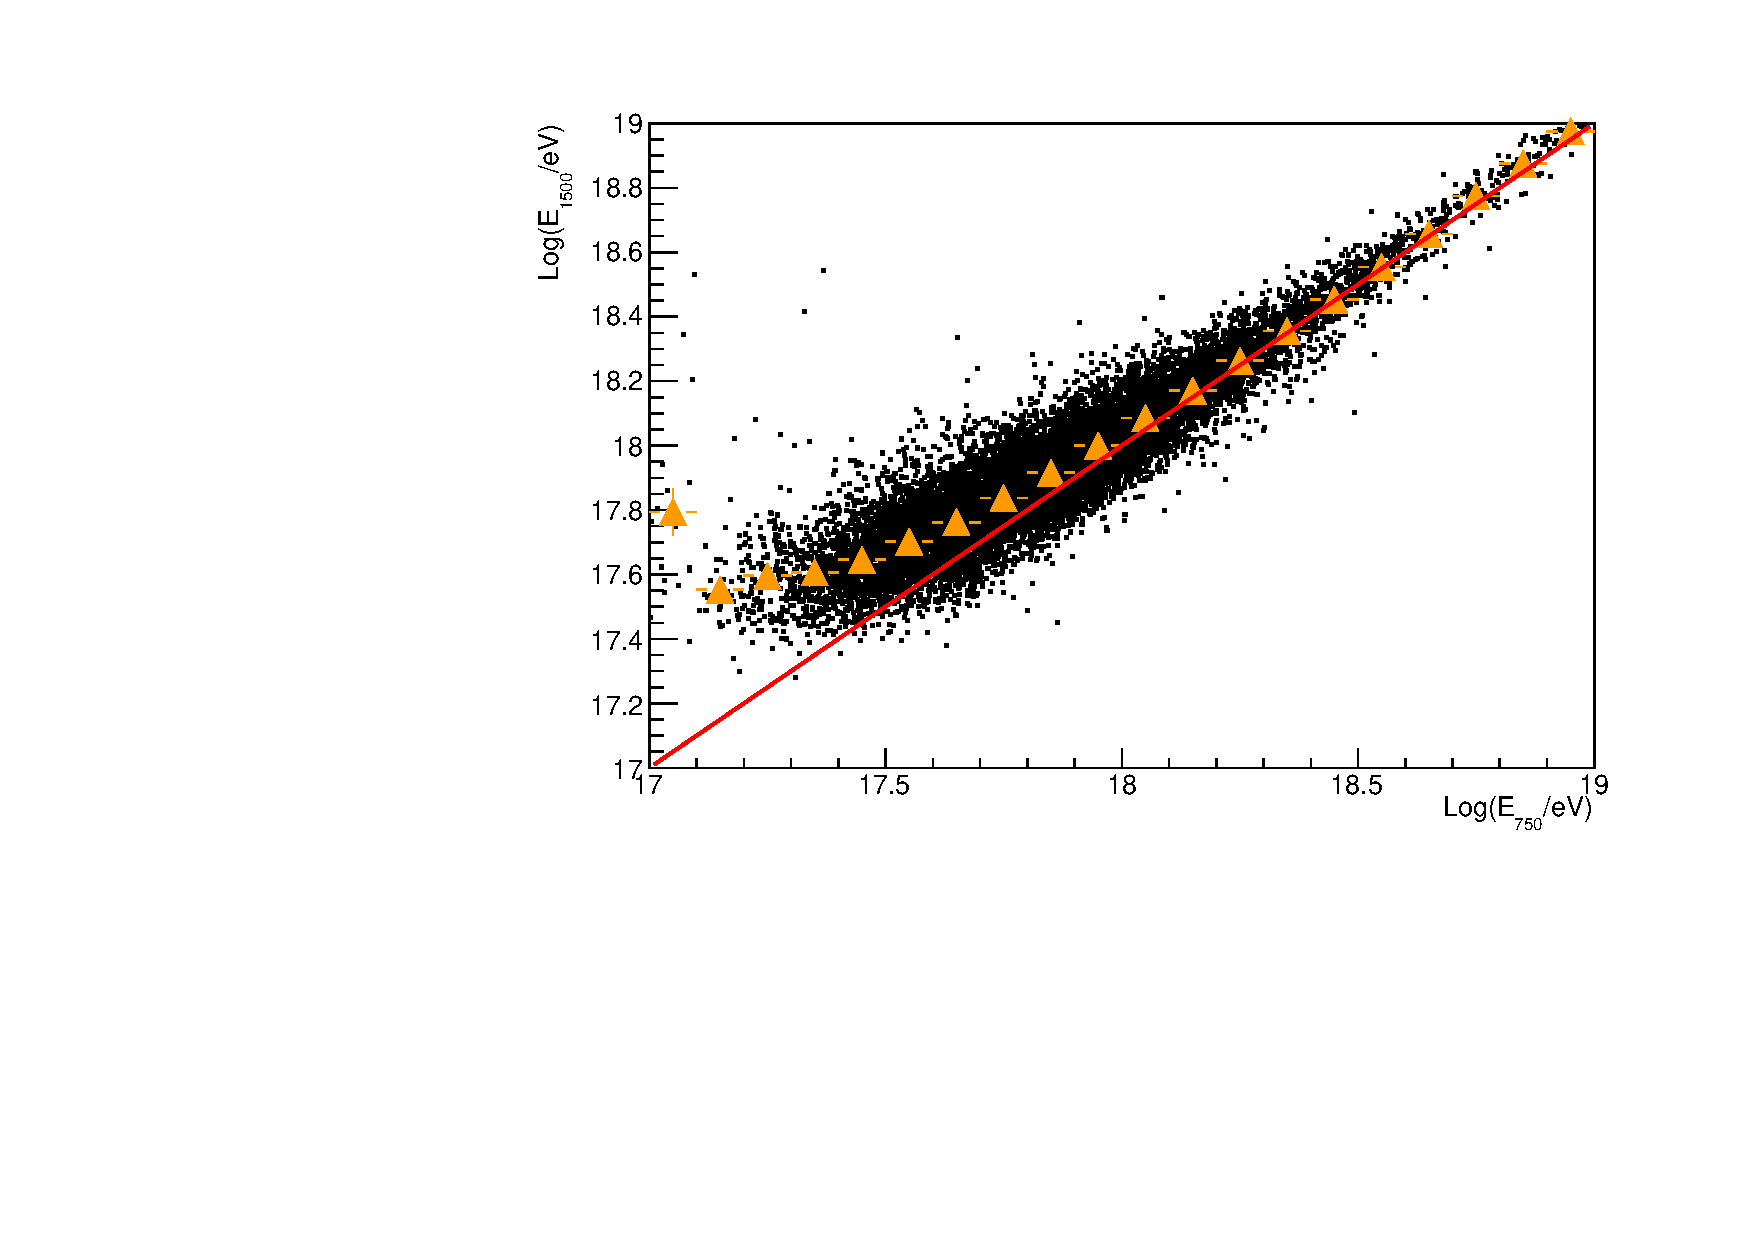
\includegraphics[width=0.5\textwidth]{plots/energy45.pdf}  
        \caption{Energy measured by the SD1500 as a function of the SD750 energy. In red it can be seen the identity function.
        \label{fig:energy}}
    \end{center}
\end{figure} 

First we proceeded with the analysis of the efficiency of the SD1500 including only the original triggers in the whole range of zenith angle. The reconstruction algorithm used for vertical events in the SD1500 ranges for $0^{\circ}\leq\theta\leq60^{\circ}$. Given that the probability of detecting an event of a given energy is binomial we used the maximum likelihood estimator (MLE) for the efficiency estimator in each bin. Also, as errors we proposed the $95\%$ confidence Wilson scored interval, which has a good coverage probability and avoids intervals higher than 1 and lower than 0 as improvements to the normal approach. Figure \ref{fig:allZenith} shows the efficiency of the SD1500 for zenith angle lower than $60^{\circ}$. 

The proposed phenomenological model of the efficiency as a function of the energy is a sigmoid function with two free parameters, $E_0$ and $b$. The election of the error function as the representation of the function is in order to make our results directly comparable with \cite{VerticalSpectrum}:

\begin{equation}
\varepsilon(E)=\frac{1}{2} + \frac{1}{2}\mathrm{erf}\left(\frac{\log_{10}(E_{750}/\mathrm{eV})-E_{0}}{b}\right)
\label{eqn:Efficiency}
\end{equation}

To fit the function we used the Minuit minimization with Root using a $\chi^2$ method obtaining parameters $E_0=17.973\pm0.004$ and $b=0.393\pm0.003$.

The full efficiency criterion for an SD array used by Auger is $\varepsilon\geq97\%$. This minimum value is used as a threshold to report events for the SD cosmic ray spectrum. For our measurement this threshold is reached for events with energy higher than $2.5\times10^{18}\eV$ which is in accordance with the value currently used.

\begin{figure}[h]
    \begin{center}
        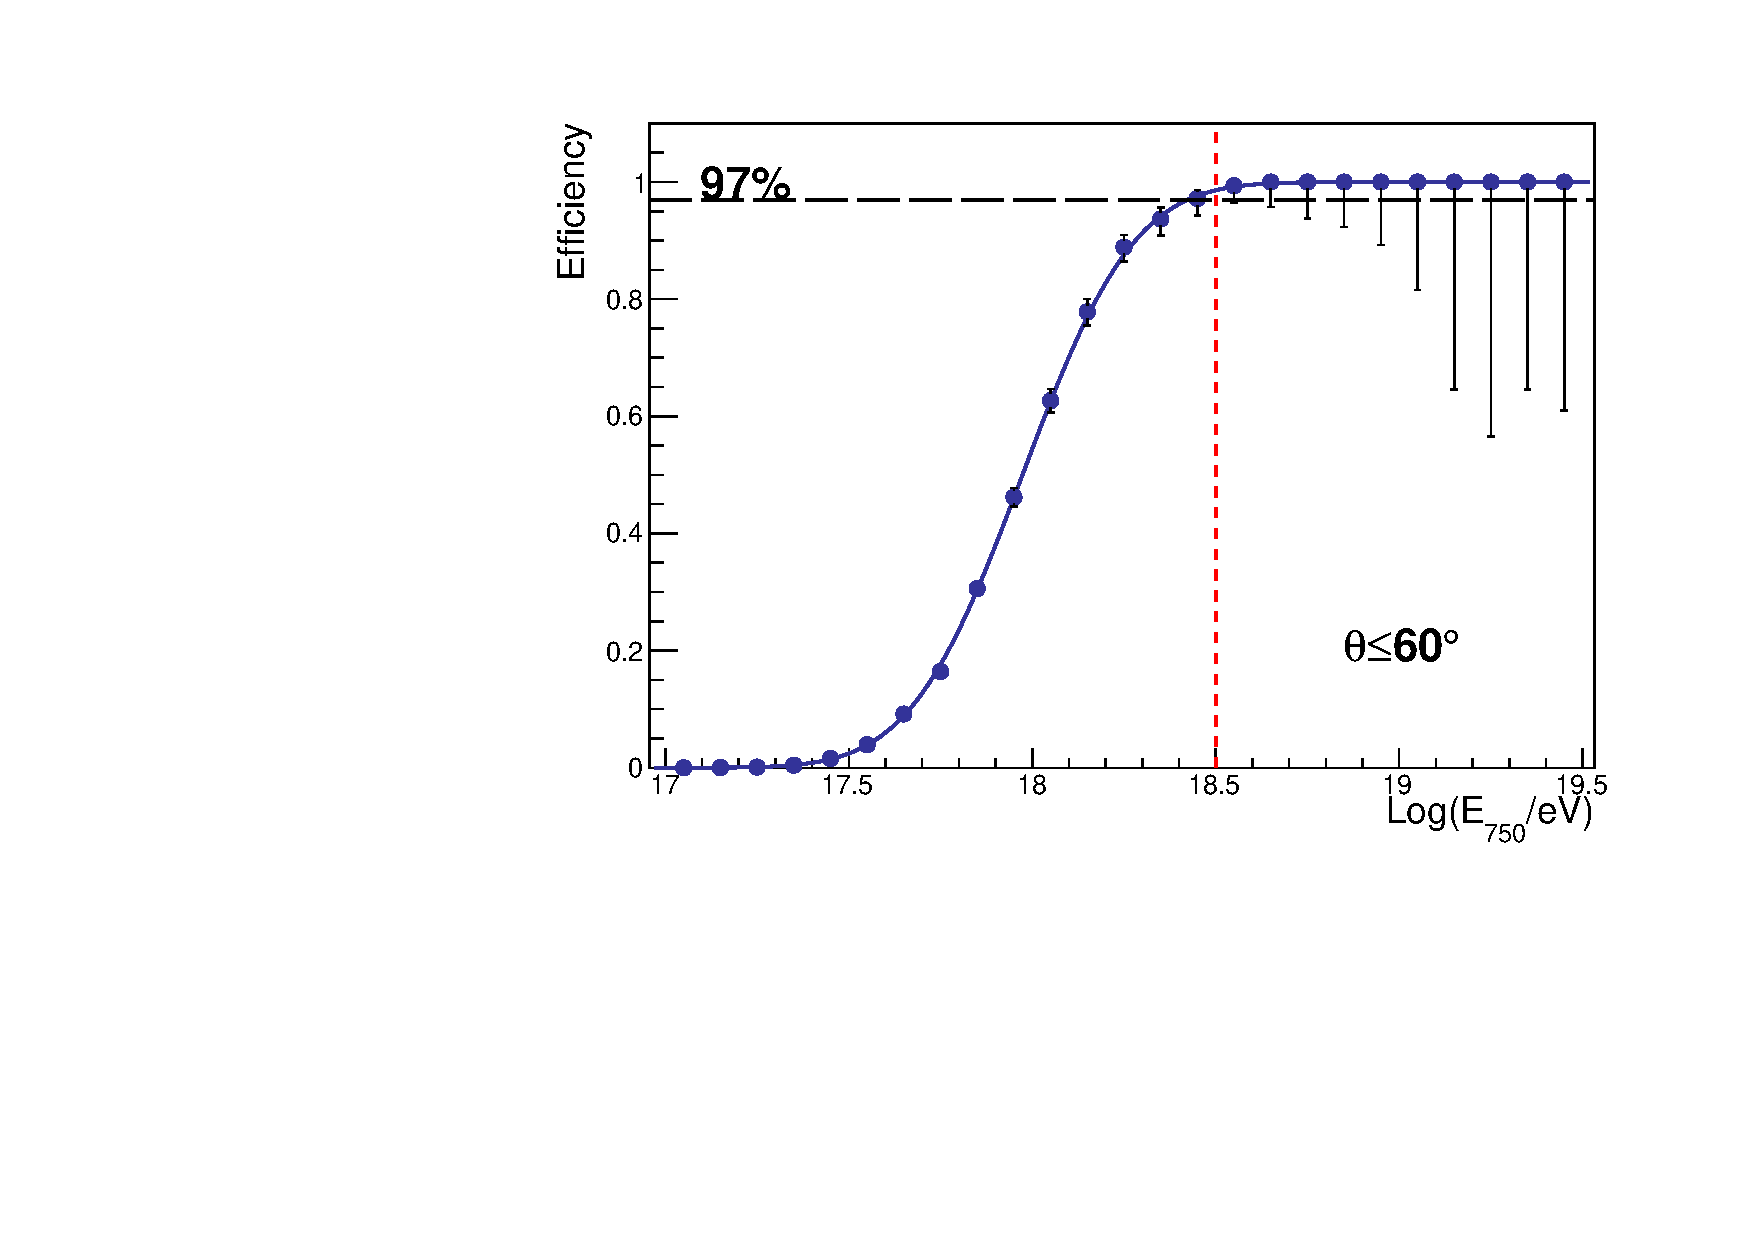
\includegraphics[width=0.5\textwidth]{plots/allZenith.pdf}  
        \caption{SD1500 efficiency measured with the SD750 event set. The error bars show the $95\%$ confidence Willson score interval. The $97\%$ efficiency threshold is reached at $2.5\times10^{18}\eV$.
        \label{fig:allZenith}}
    \end{center}
\end{figure}


%%%%%%%%%%%%%%%%%%%%%%%%%%%%%%Zenith Dependence%%%%%%%%%%%%%%%%%%%%%%%%%%%%%%%%%


\section{Zenith angle dependence of the efficiency}
\label{sec:zenith}

The next step is to analyze the dependency of the efficiency with the zenith angle of the events. We divided the events with zenith angles $\leq60^{\circ}$ in twelve zenith bins equispaced in $\sin^2(\theta)$ in order to have approximately the same exposure. Based on \cite{VerticalSpectrum} we propose a combined model of the efficiency consisting in a sigmoid function, just like Eq. \ref{eqn:Efficiency} but including the dependency on the zenith angle in the parameters $E_0$ and $b$:

\begin{equation}
\varepsilon(E,\theta)=\frac{1}{2} + \frac{1}{2}\mathrm{erf}\left(\frac{\log_{10}(E_{750}/\mathrm{eV})-E_{0}(\theta)}{b(\theta)}\right)
\label{eqn:EffiZenith}
\end{equation}

In order to see the functional form of $E_0(\theta)$ and $b(\theta)$ we propose a preliminary analysis where the efficiency is measured for each $\sin^2(\theta)$ bin separately and then the parameters are plotted, as is shown in figure \ref{fig:parameters}. It can be seen a quadratic dependency of $E_0$ on $\sin^2(\theta)$ while for $b(\theta)$, two models are proposed, one of constant $b$ and other linear in $\sin^2(\theta)$. In consequence two parametrizations of the efficiency as a function of the energy and the zenith angle are proposed. One of 4 parameters with $E_0(\theta)=p_0 + p_1\sin^2(\theta) + p_2\sin^4(\theta)$ and $b=b_0$ and one of 5 parameters with the same $E_0$ but $b=b_0+b_1\sin^2(\theta)$. With the fitted parameters for the single bins as initial values, we made a simultaneous $\chi^2$ fit of the efficiency as a function of the energy and the zenith angle for the 4 parameter and the 5 parameter models. Results are shown in \ref{tab:param}.

In order to see our results, we evaluated the fits in the center of the zenith angle bin. \ref{fig:zenithSingle} shows the efficiency as a function of the energy for the bin $56.0 \leq \theta \leq 60.0$ together with the preliminary fit and the 4 and 5 parameter model. It can be seen that for this bin, the 5 parameters model offers a better description of the data. \ref{fig:zenith} shows the efficiency and the three fittings for all the twelve zenith bins. For the vertical bins, both the 4 and 5 parameter fits show accordance with the measured efficiency but for the more inclined events, the 5 parameter description adjust better the data. In consequence, our proposed model of the efficiency is:

\begin{equation}
\varepsilon(E,\theta)=\frac{1}{2}\left(1+\mathrm{erf}\left(\frac{\log_{10}(E/\mathrm{eV})-(p_0+p_1\sin^2(\theta)+p_2\sin^4(\theta))}{b_0+b_1\sin^2(\theta)}\right)\right)
\label{eqn:fitting}
\end{equation}
with $p_0=18.03$ $p_1=-0.91$, $p_2=1.45$, $b_0=0.336$, $b_1=-0.068$.

\begin{figure}[]
    \center
    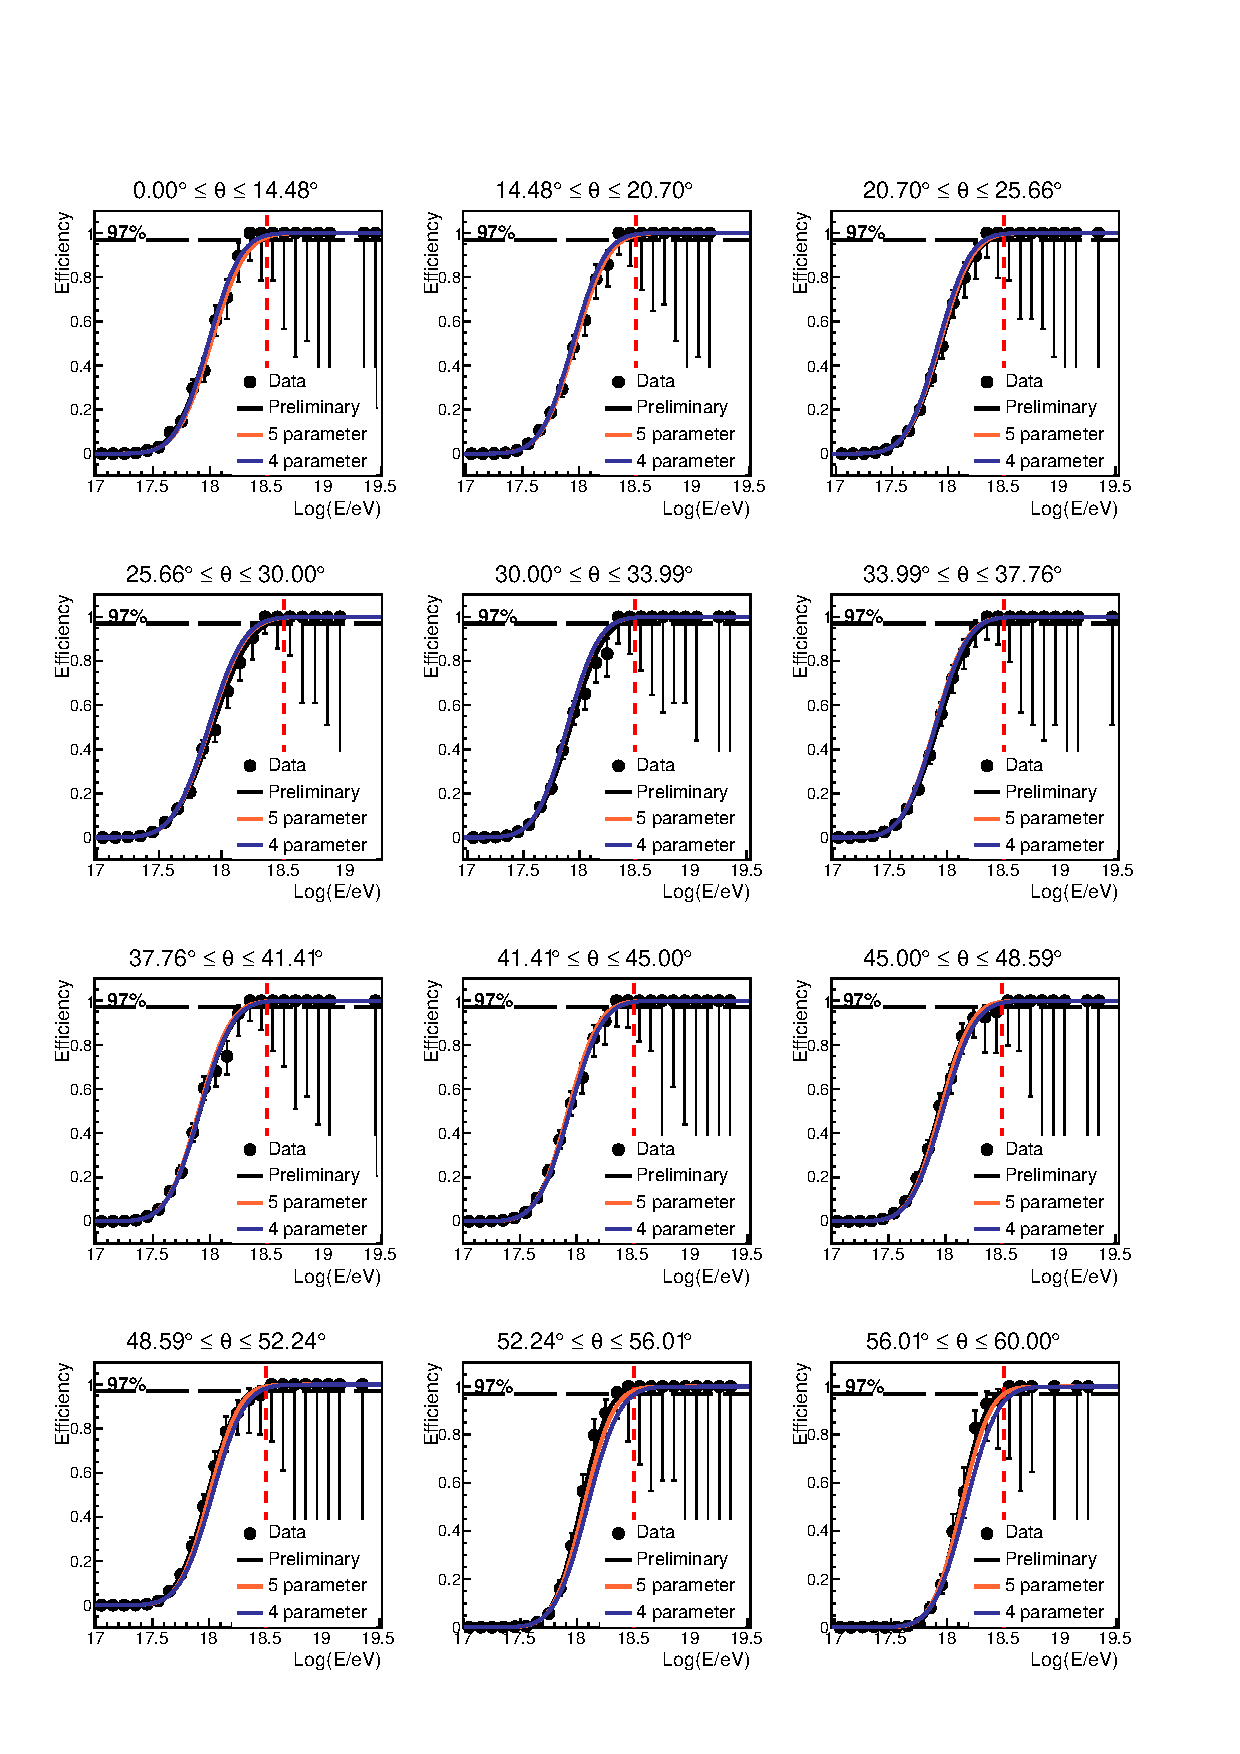
\includegraphics[height=0.95\textheight]{plots/EfficiencyZenith.pdf}
    \caption{SD1500 efficiency for zenith angle bins and the 4 and 5 parameter fittings proposed together with the preliminary fit.
    \label{fig:zenith}}
\end{figure}



\begin{figure}[h]
    \begin{center}
        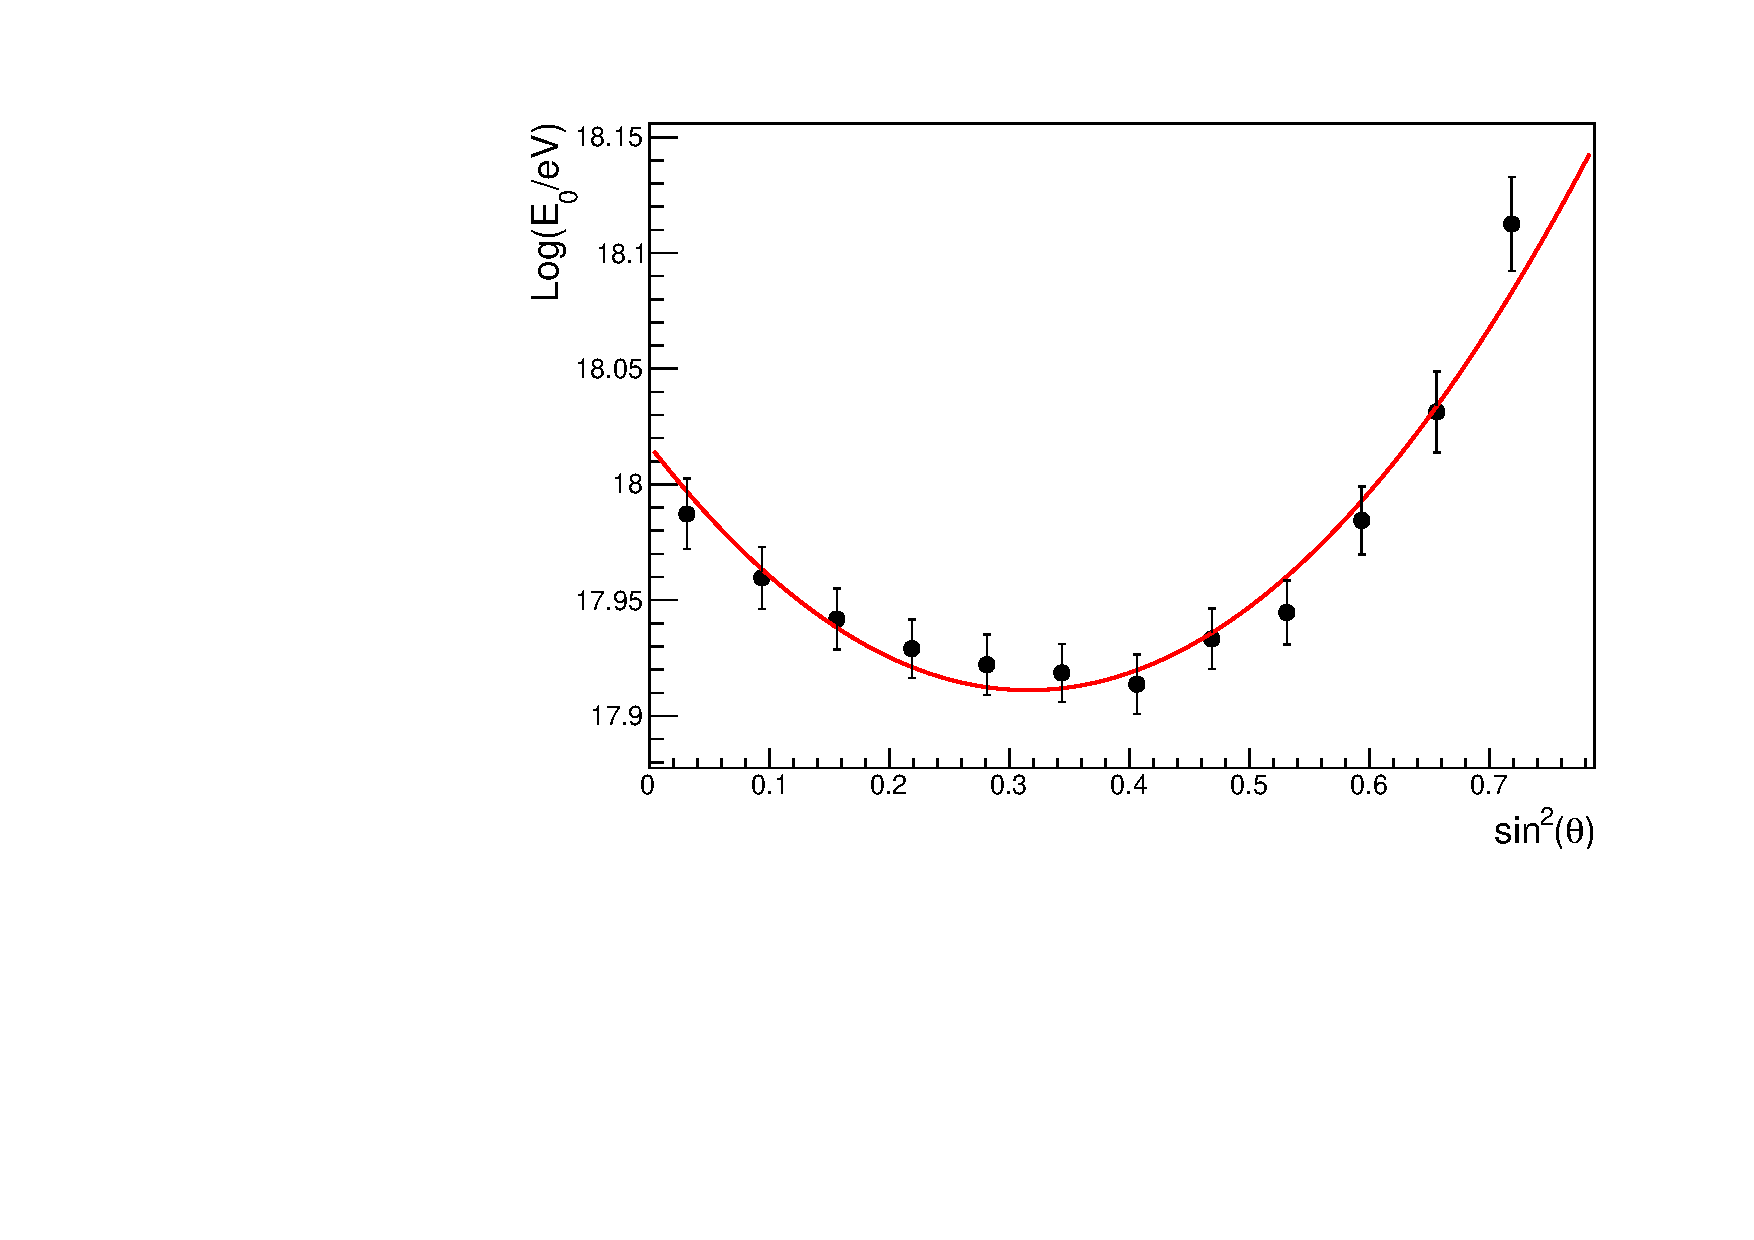
\includegraphics[width=0.49\textwidth]{plots/E0.pdf}
        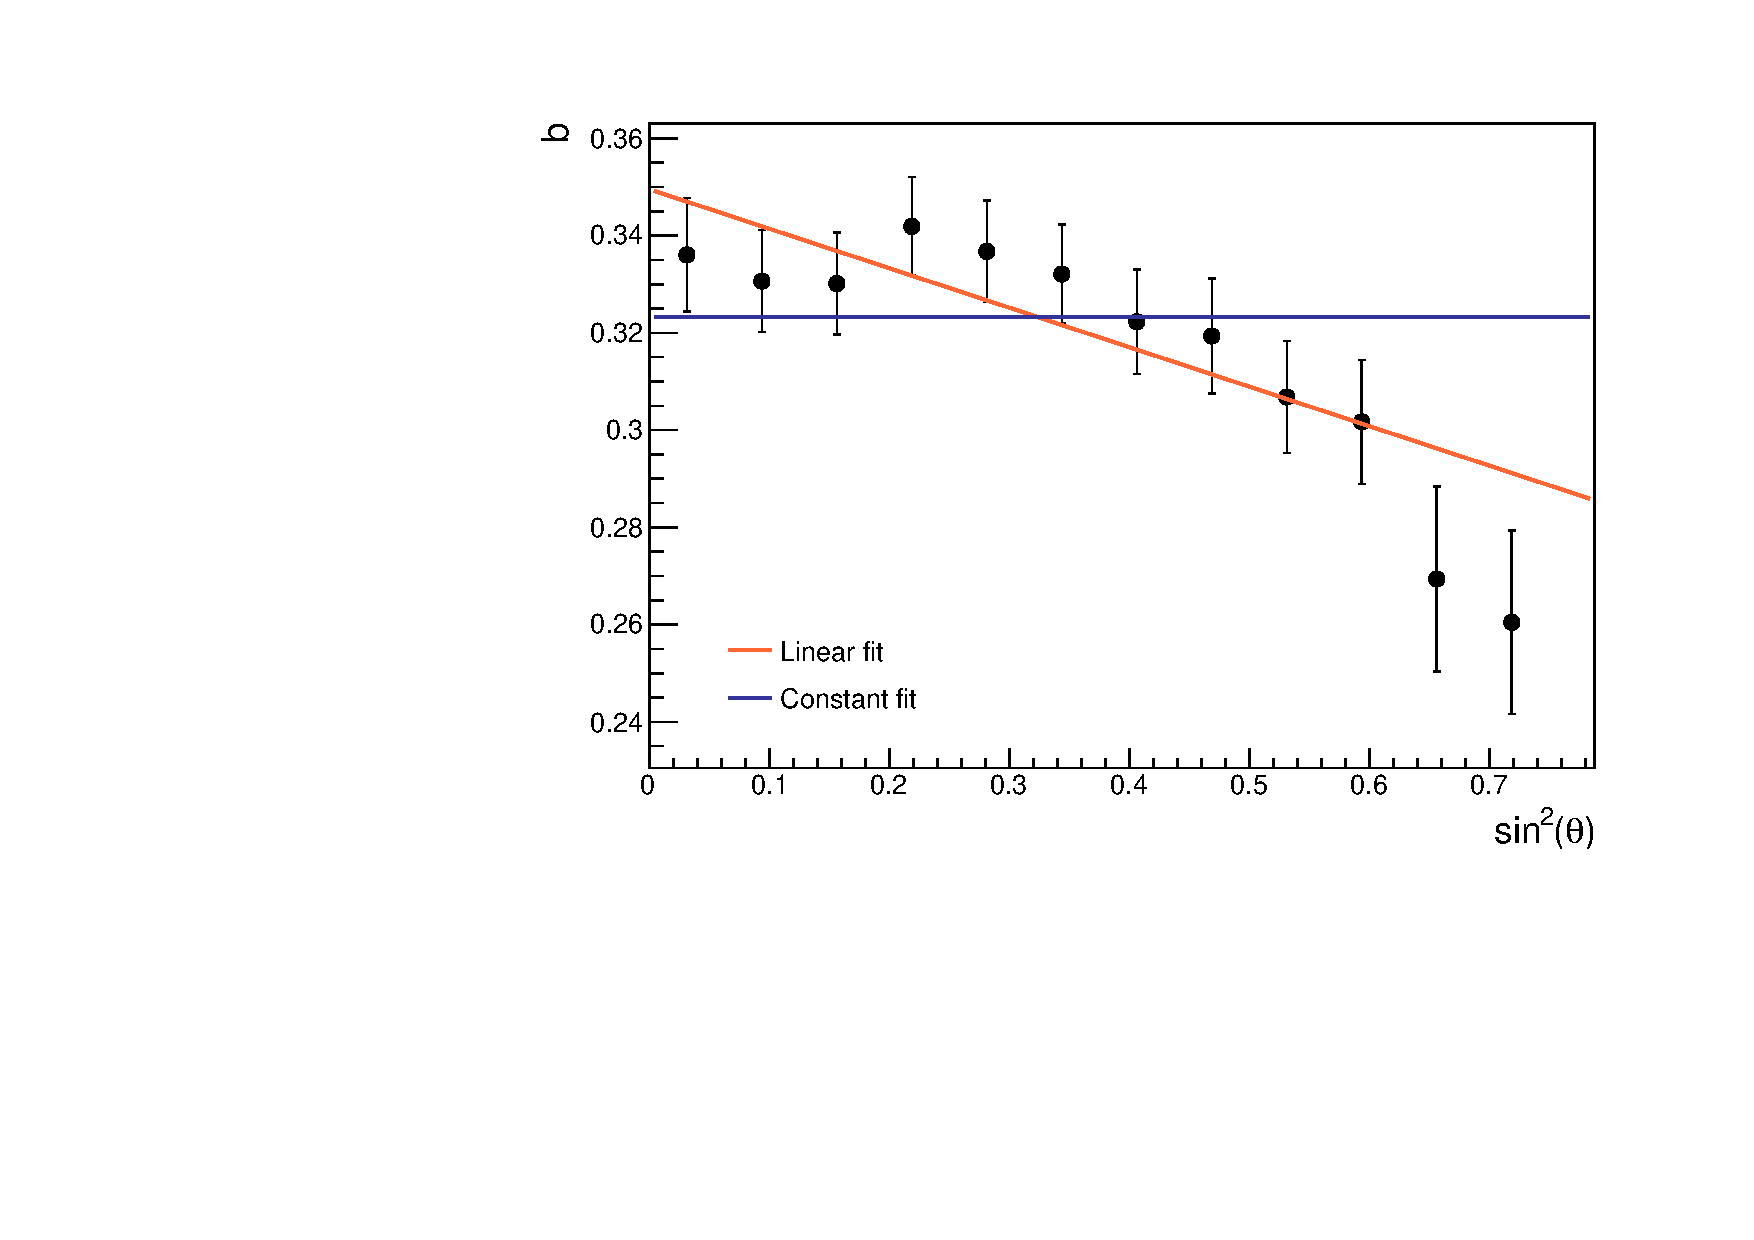
\includegraphics[width=0.49\textwidth]{plots/b.pdf}
        \caption{Parameter dependency with $\sin^2(\theta)$ for the preliminary fit. $E_0$ shows a quadratic dependence and $b$ is modeled by a constant function and a linear function.
        \label{fig:parameters}}
    \end{center}
\end{figure} 



\begin{figure}[h]
    \begin{center}
        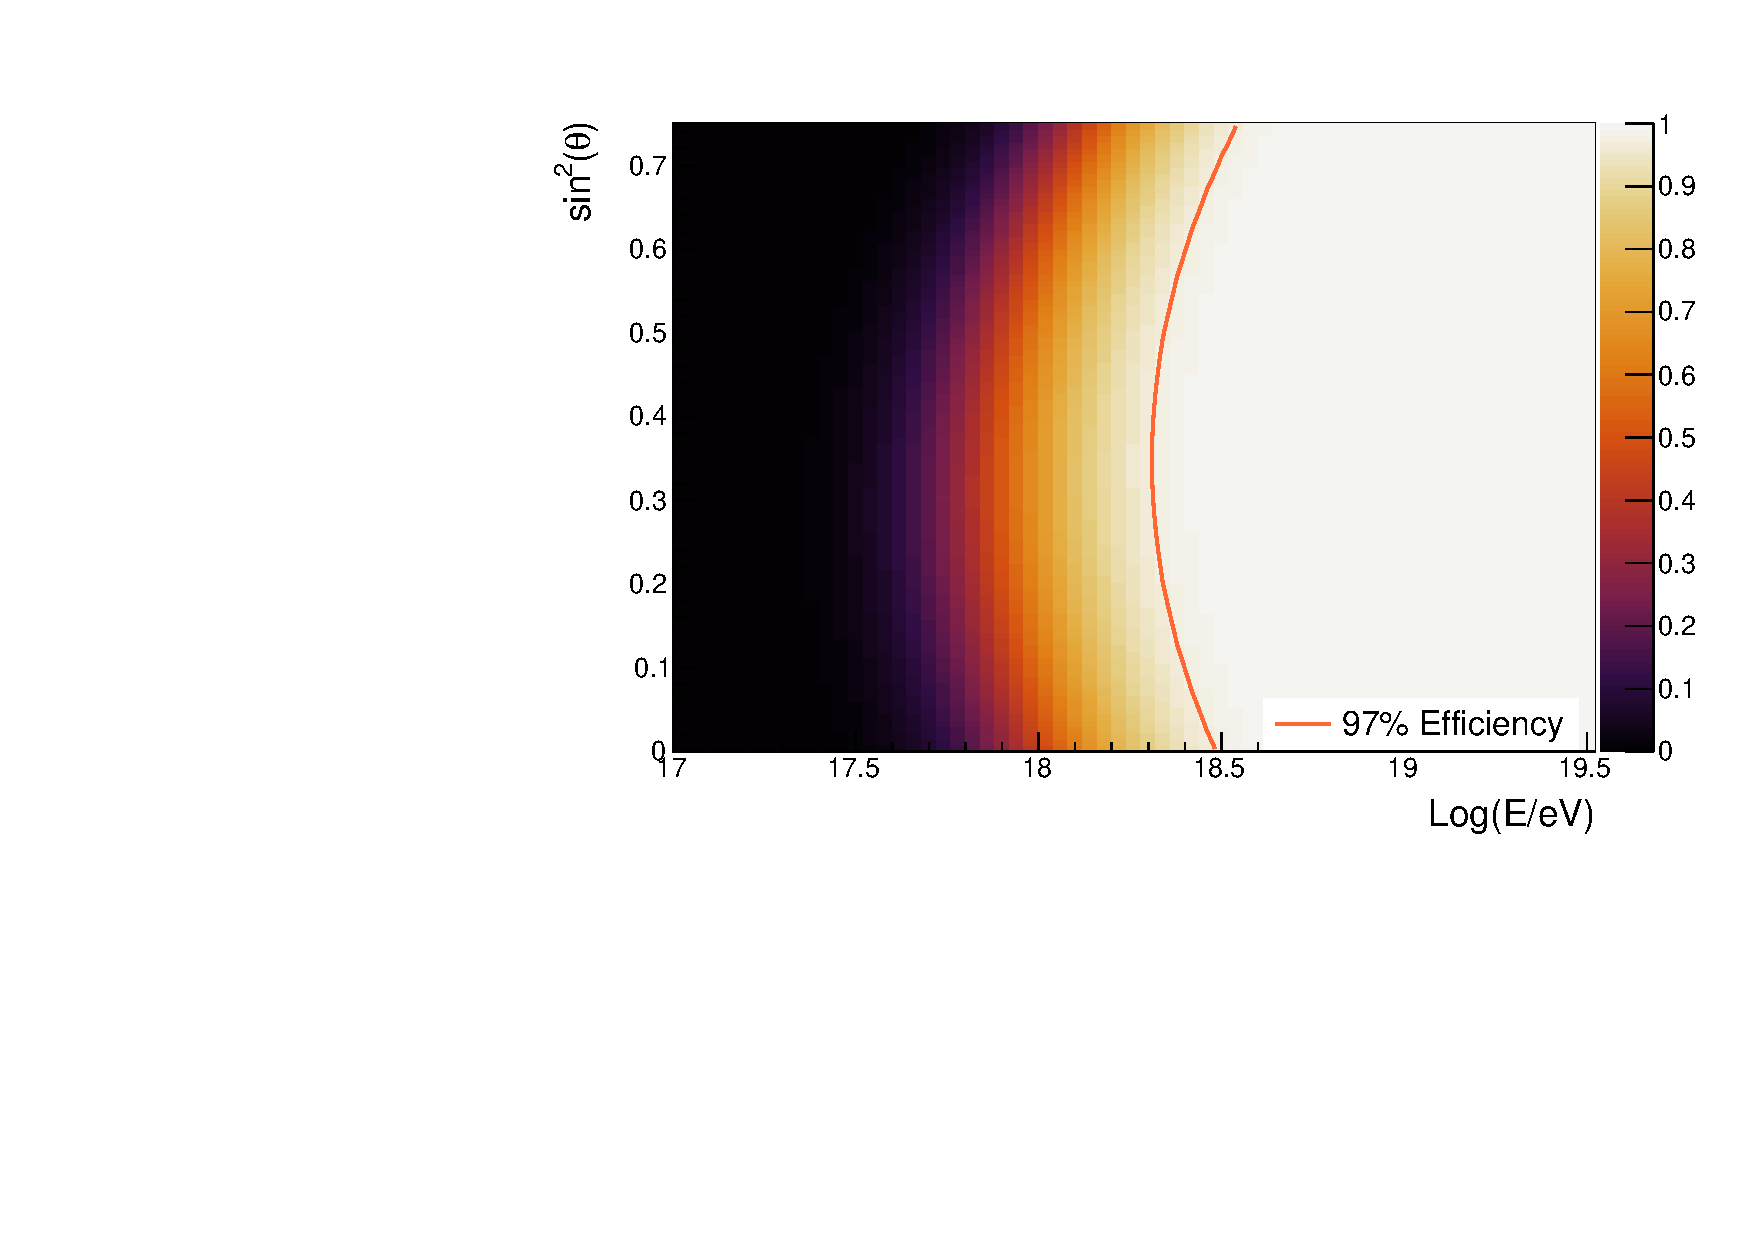
\includegraphics[width=0.7\textwidth]{plots/Surface.pdf}
        \caption{Efficiency as function of the Energy and zenith angle and the $97\%$ surface level .
        \label{fig:surface}}
    \end{center}
\end{figure}  

\section{Efficiency of the 1500-metre array with the inclusion of the new triggers}
\label{sec:new}

\begin{figure}[h]
    \begin{center}
        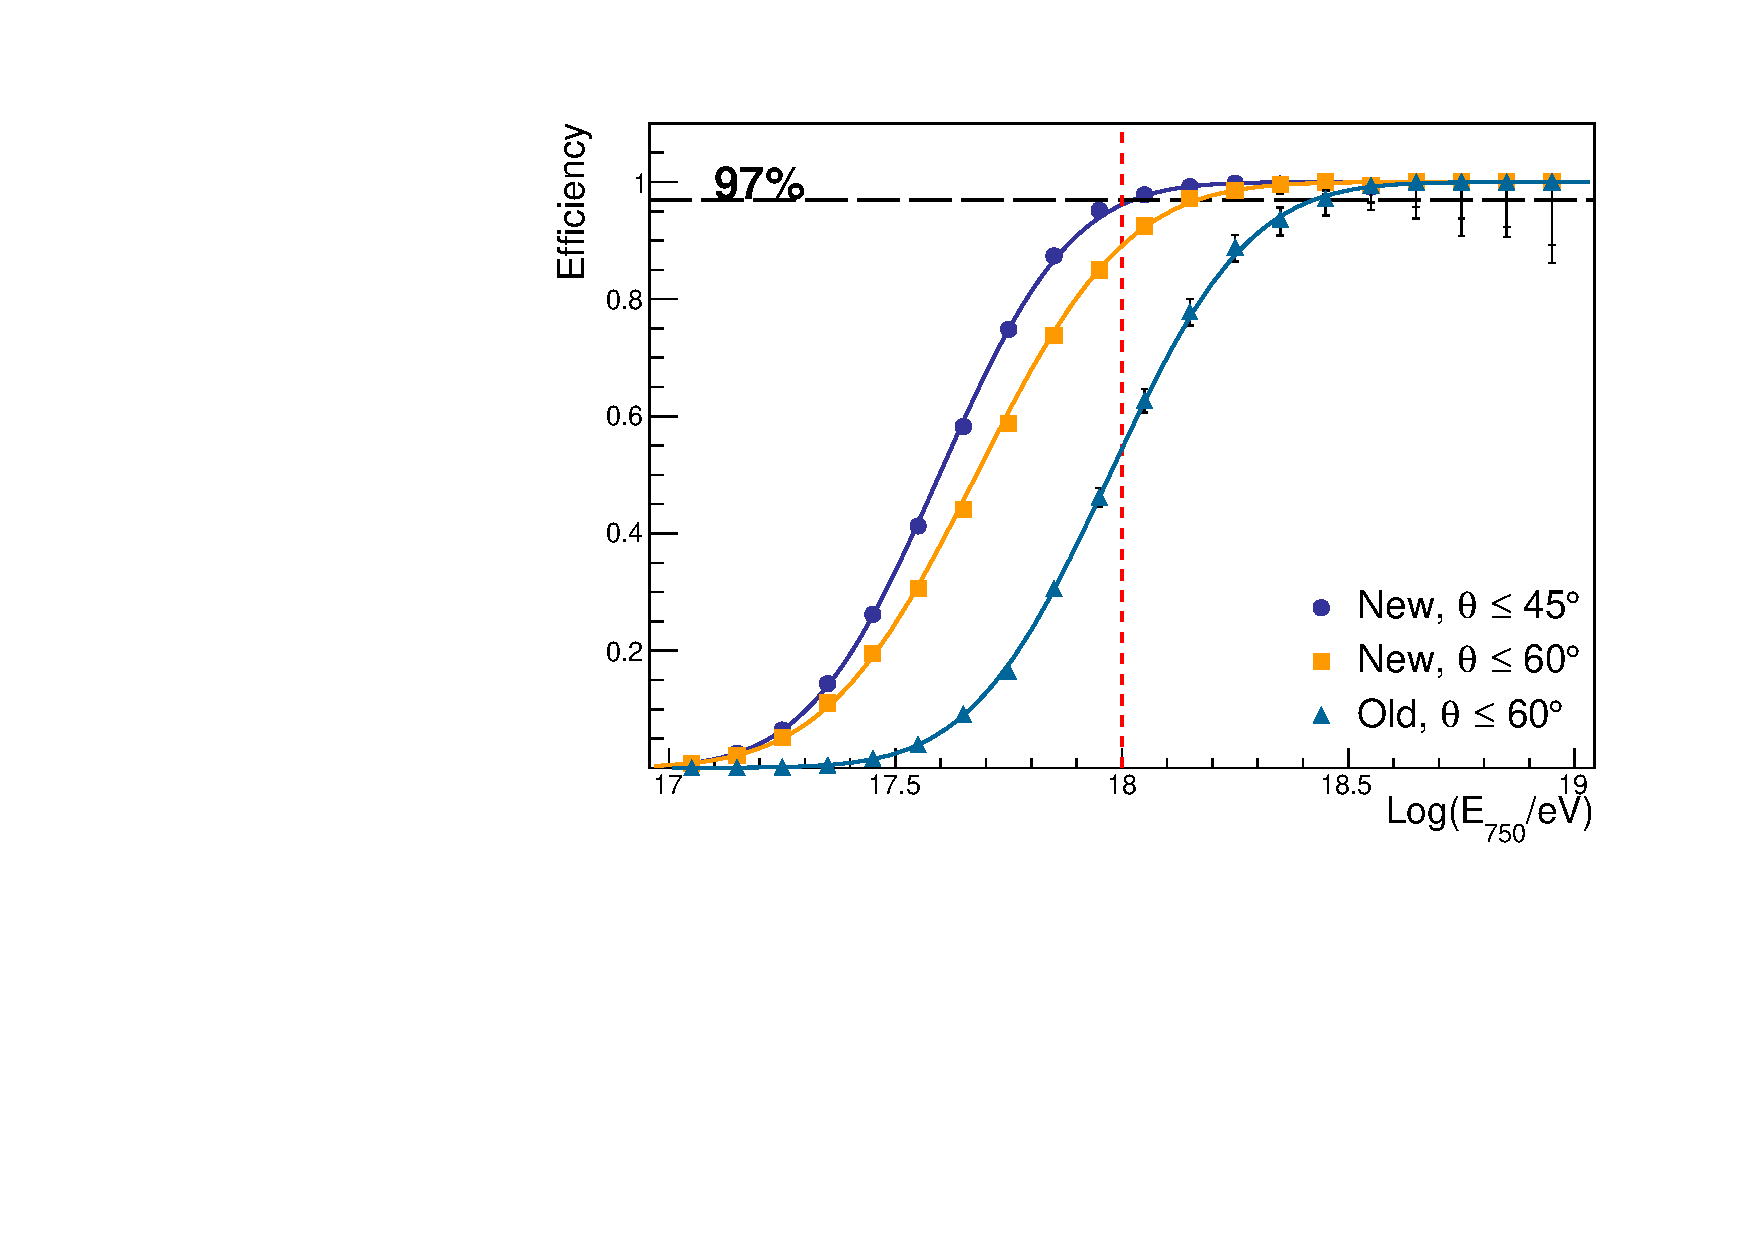
\includegraphics[width=0.7\textwidth]{plots/NewCut.pdf}
        \caption{SD1500 efficiency including the new triggers for $\theta\leq60^\circ$ and $\theta\leq45^\circ$. The $97\%$ efficiency threshold is reached at $10^{18.2}\eV$ and $10^{18}\eV$ respectively.
        \label{fig:NewCut}}
    \end{center}
\end{figure}


\section{Efficiency correction of the SD-1500 Spectrum}
\label{sec:spectrum}

%%

\begin{figure}[hb]
    \begin{center}
        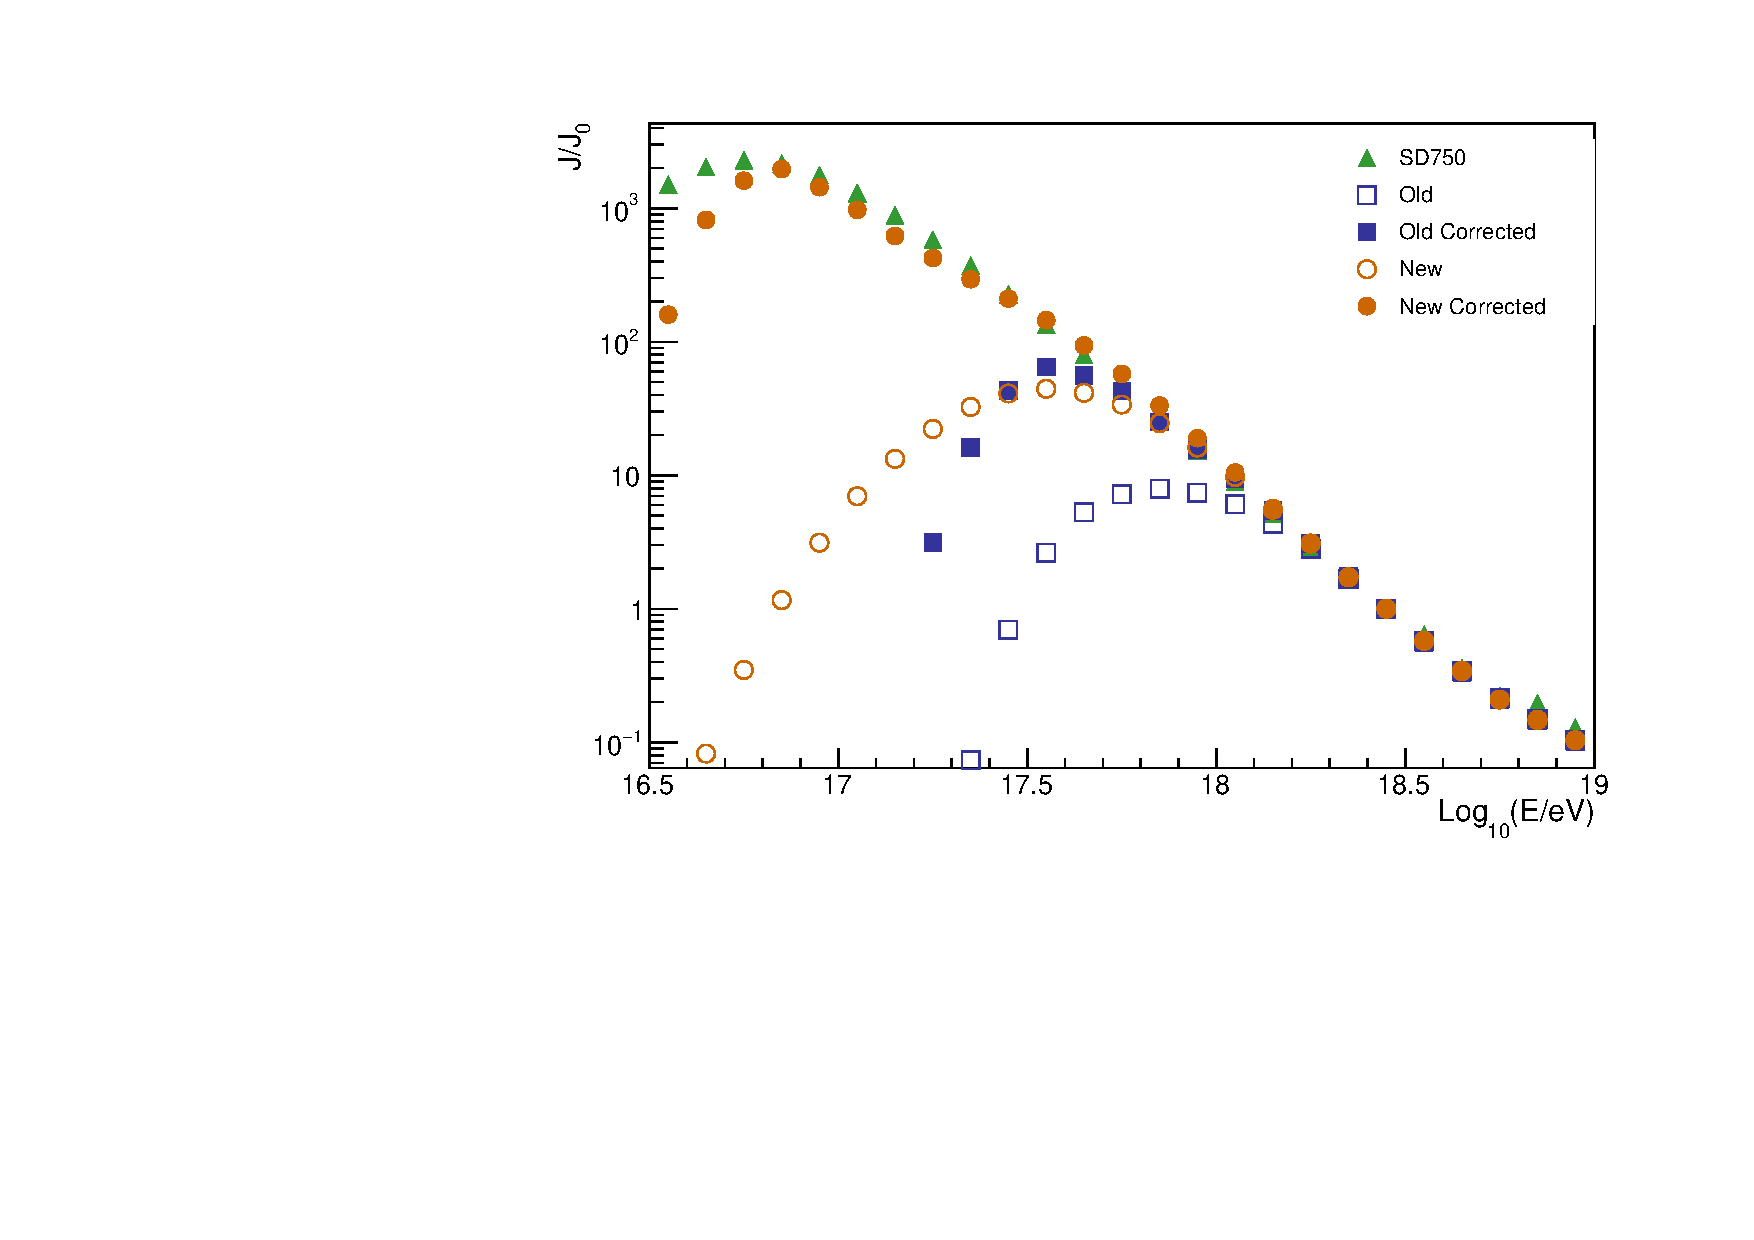
\includegraphics[width=0.7\textwidth]{plots/spectrum.pdf}
        \caption{Raw flux measured by the SD1500 using old and new triggers and it's efficiency correction. The fluxes were normalized to $J_{18.2}=1$.
        \label{fig:flux}}
    \end{center}
\end{figure}

\begin{figure}[h]
    \begin{center}
        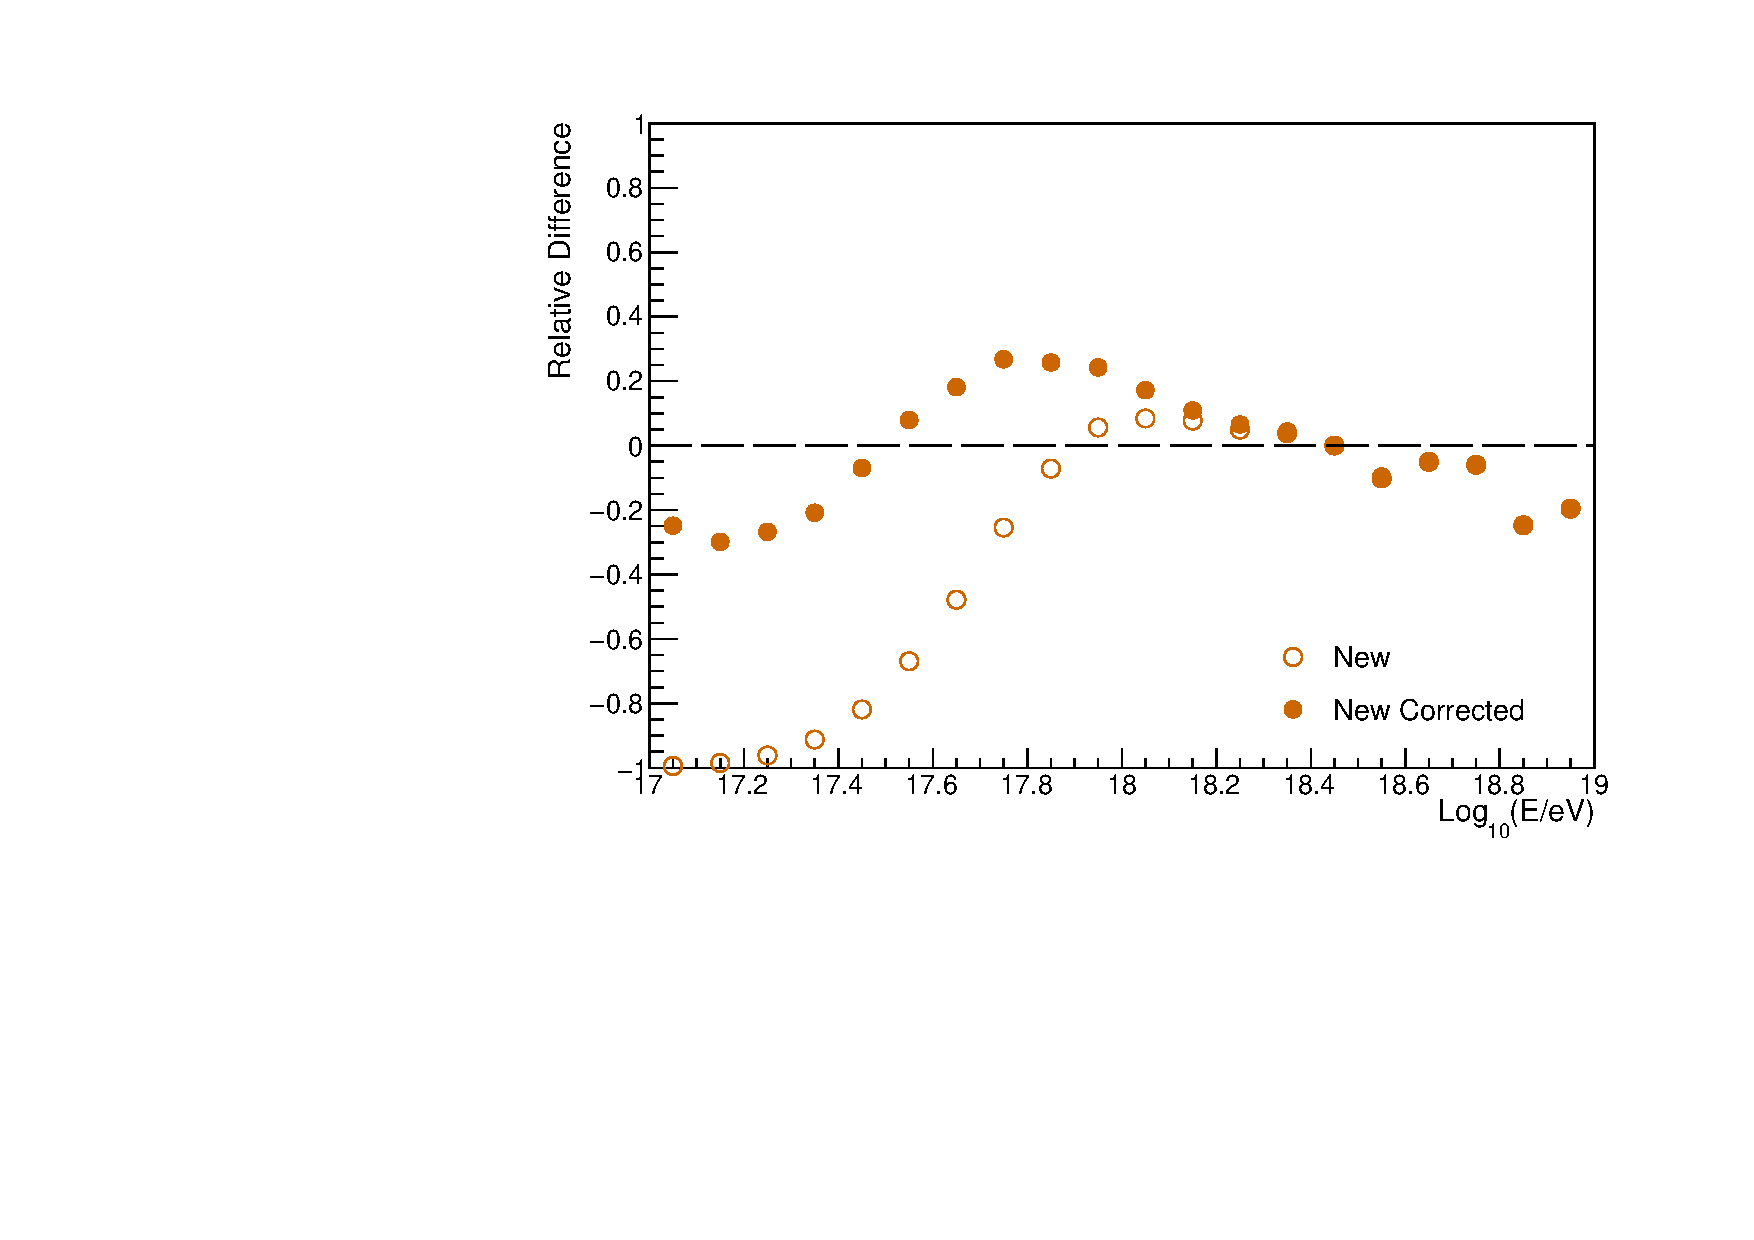
\includegraphics[width=0.7\textwidth]{plots/NewDifference.pdf}
        \caption{Relative difference between SD1500 flux and the SD750 for the old trigger reconstruction and after efficiency correction.
        \label{fig:difference}}
    \end{center}
\end{figure} 


\section*{Appendix: New Triggers}

\begin{figure}[h]
    \begin{center}
        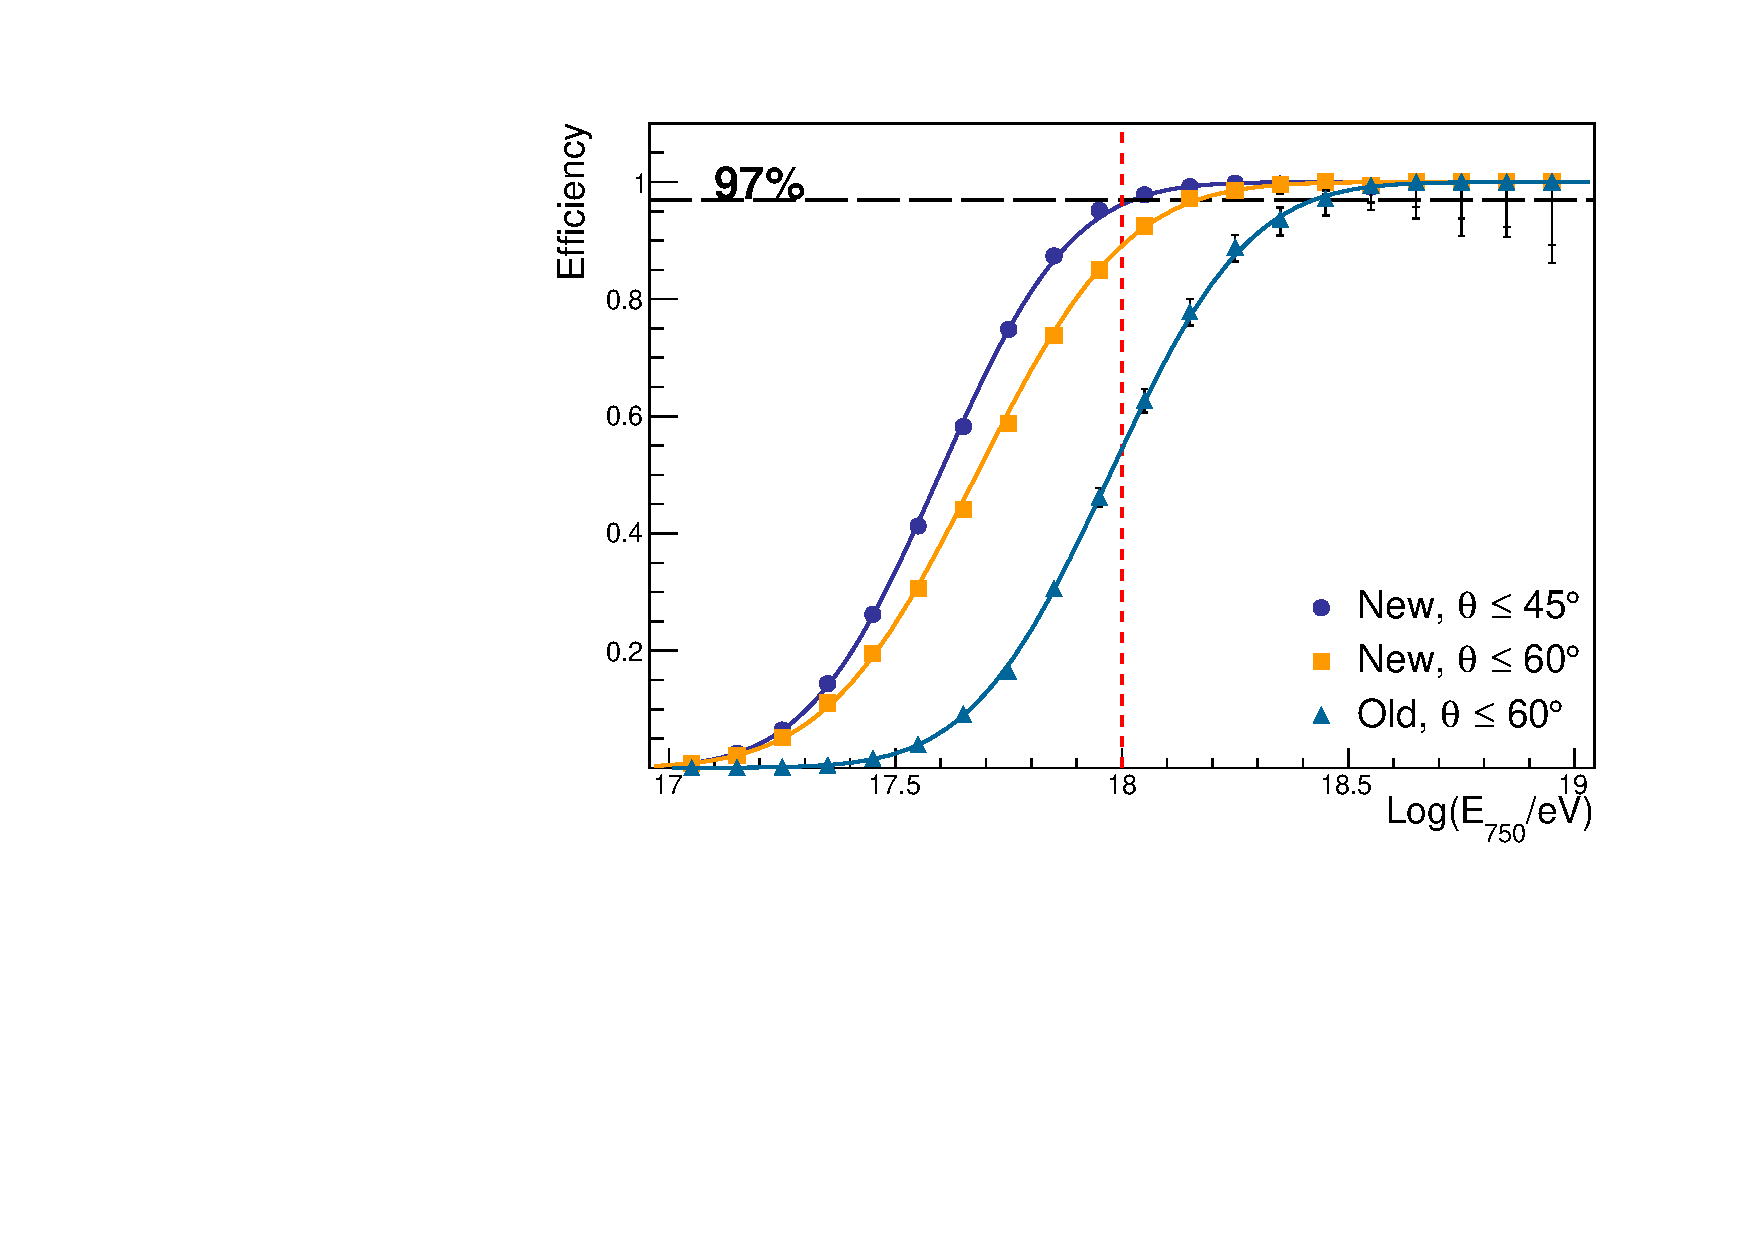
\includegraphics[width=0.7\textwidth]{plots/NewCut.pdf}  
        \caption{SD1500 efficiency for events reconstructed with the incorporation of the new triggers. The minimum energy bin above the $97\%$ efficiency threshold is $10^{18.2}\eV$
        \label{fig:allZenithNew}}
    \end{center}
\end{figure}

\begin{figure}[p]
    \begin{center}
        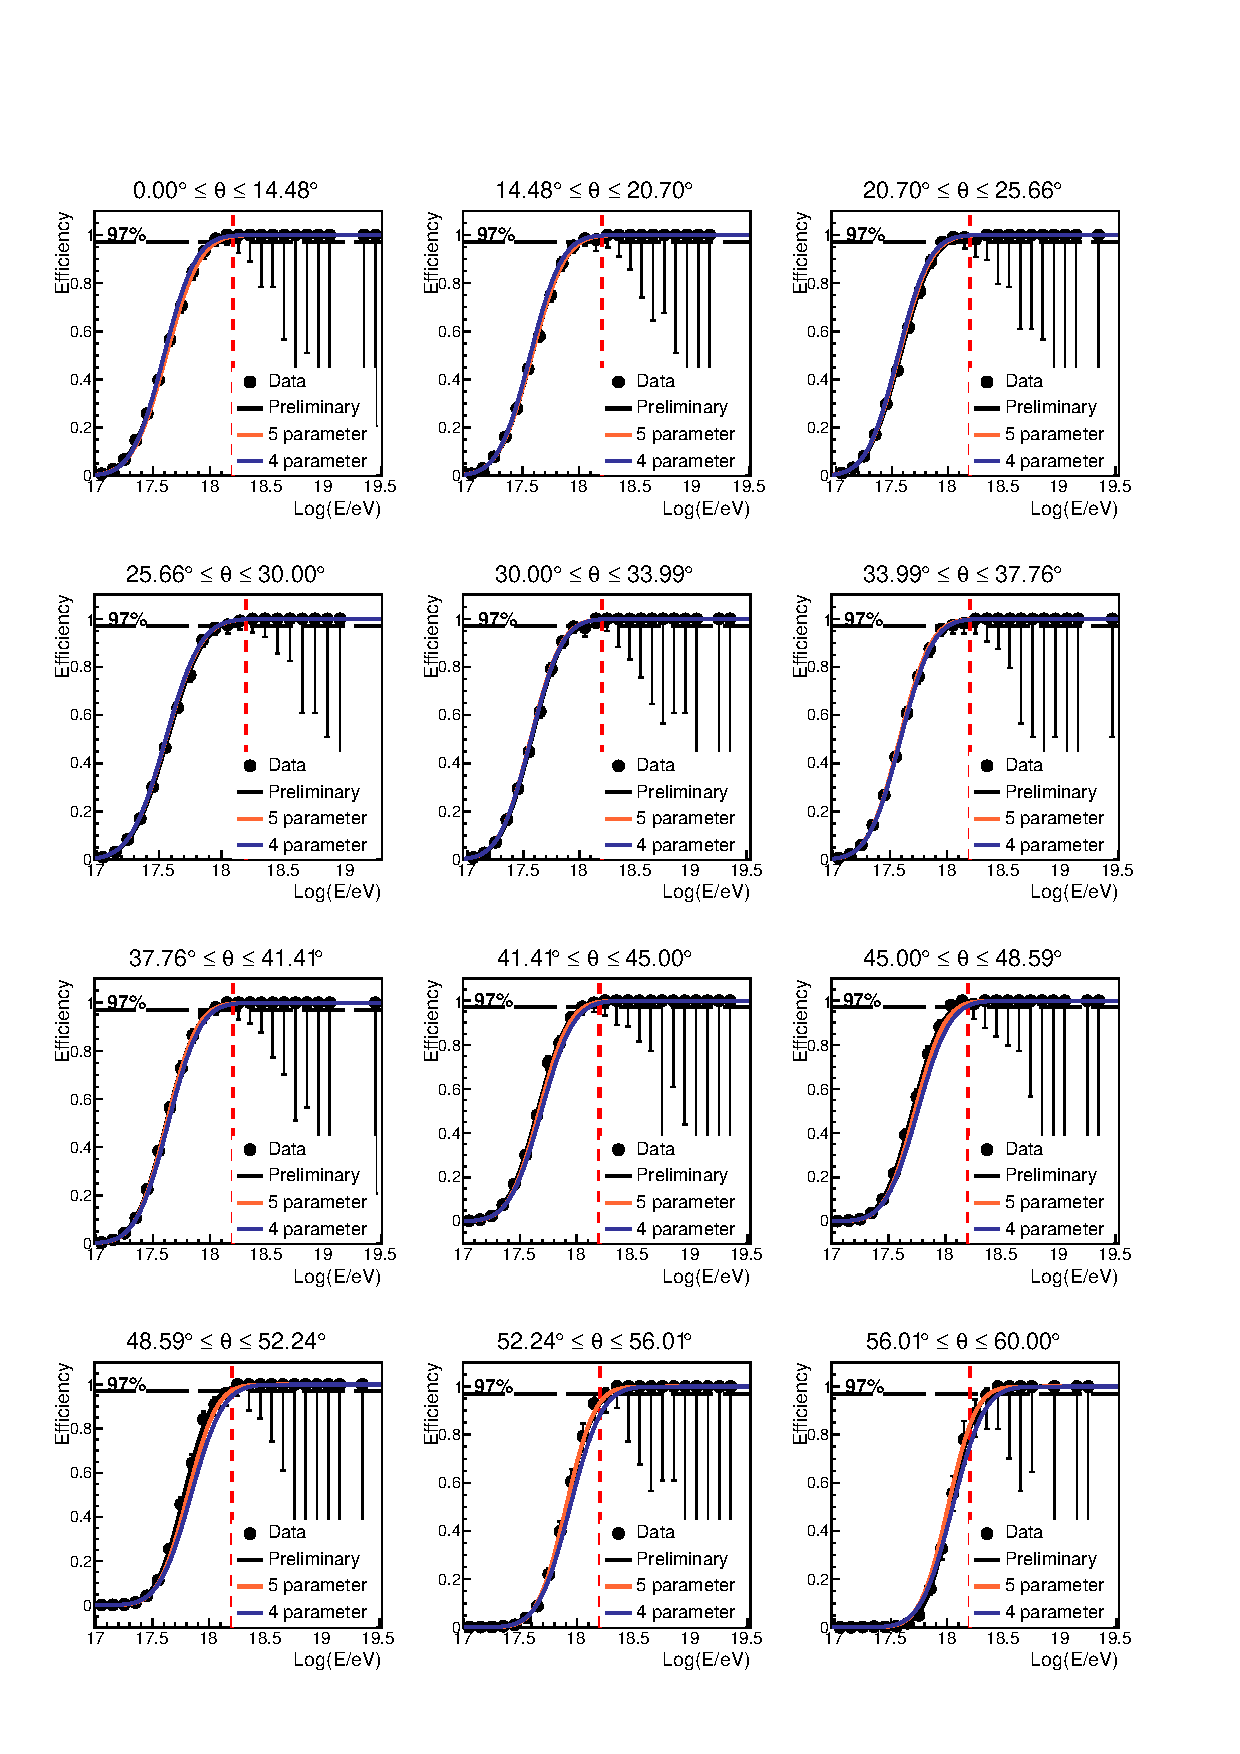
\includegraphics[height=0.97\textheight]{plots/EfficiencyZenithNew.pdf}
        \caption{Efficiency for the zenith angle bins for events reconstructed including the new triggers and it's parametrizations.
        \label{fig:zenithNew}}
    \end{center}
\end{figure}

\begin{figure}[h]
    \begin{center}
        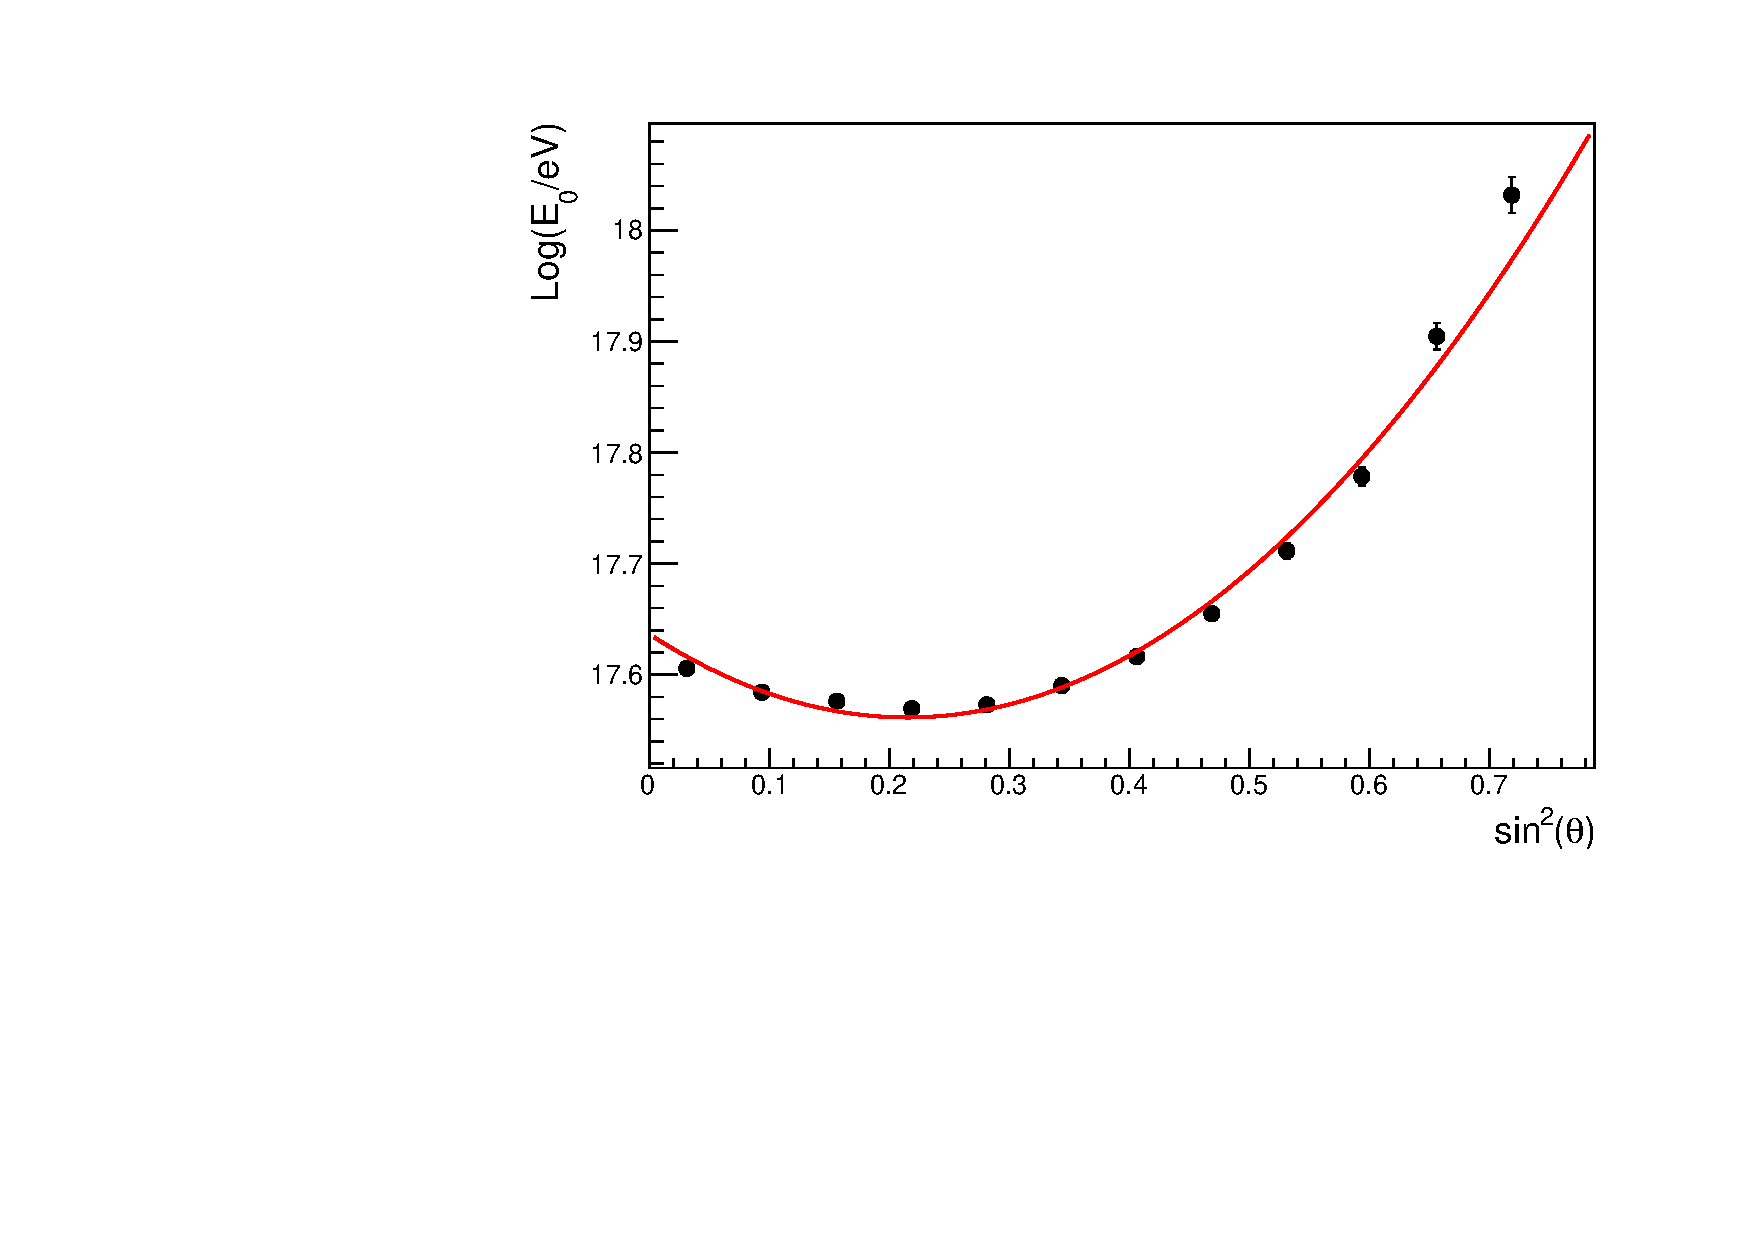
\includegraphics[width=0.49\textwidth]{plots/E0New.pdf}
        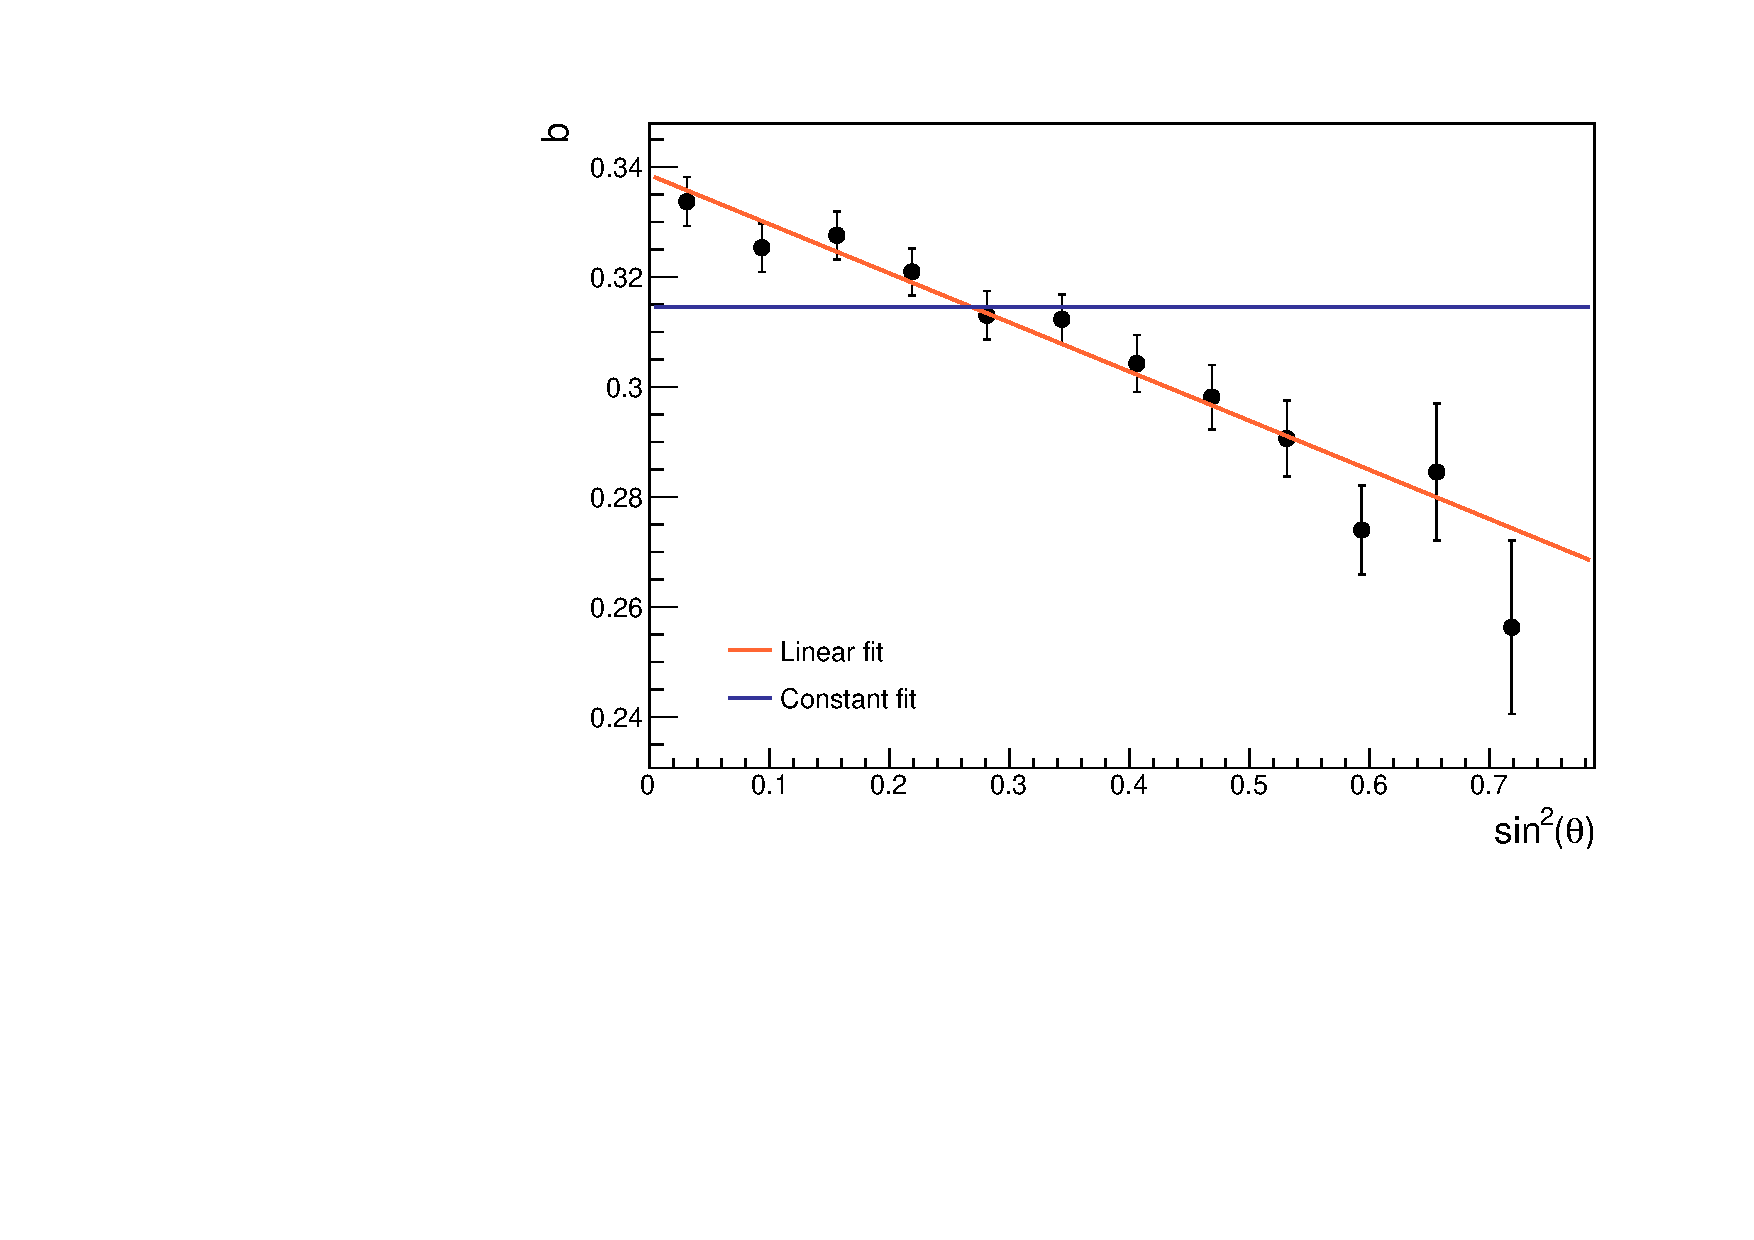
\includegraphics[width=0.49\textwidth]{plots/bNew.pdf}
        \caption{Preliminary fit parameter dependency on $\sin^2(\theta)$.
        \label{fig:parametersNew}}
    \end{center}
\end{figure} 

\begin{figure}[h]
    \begin{center}
        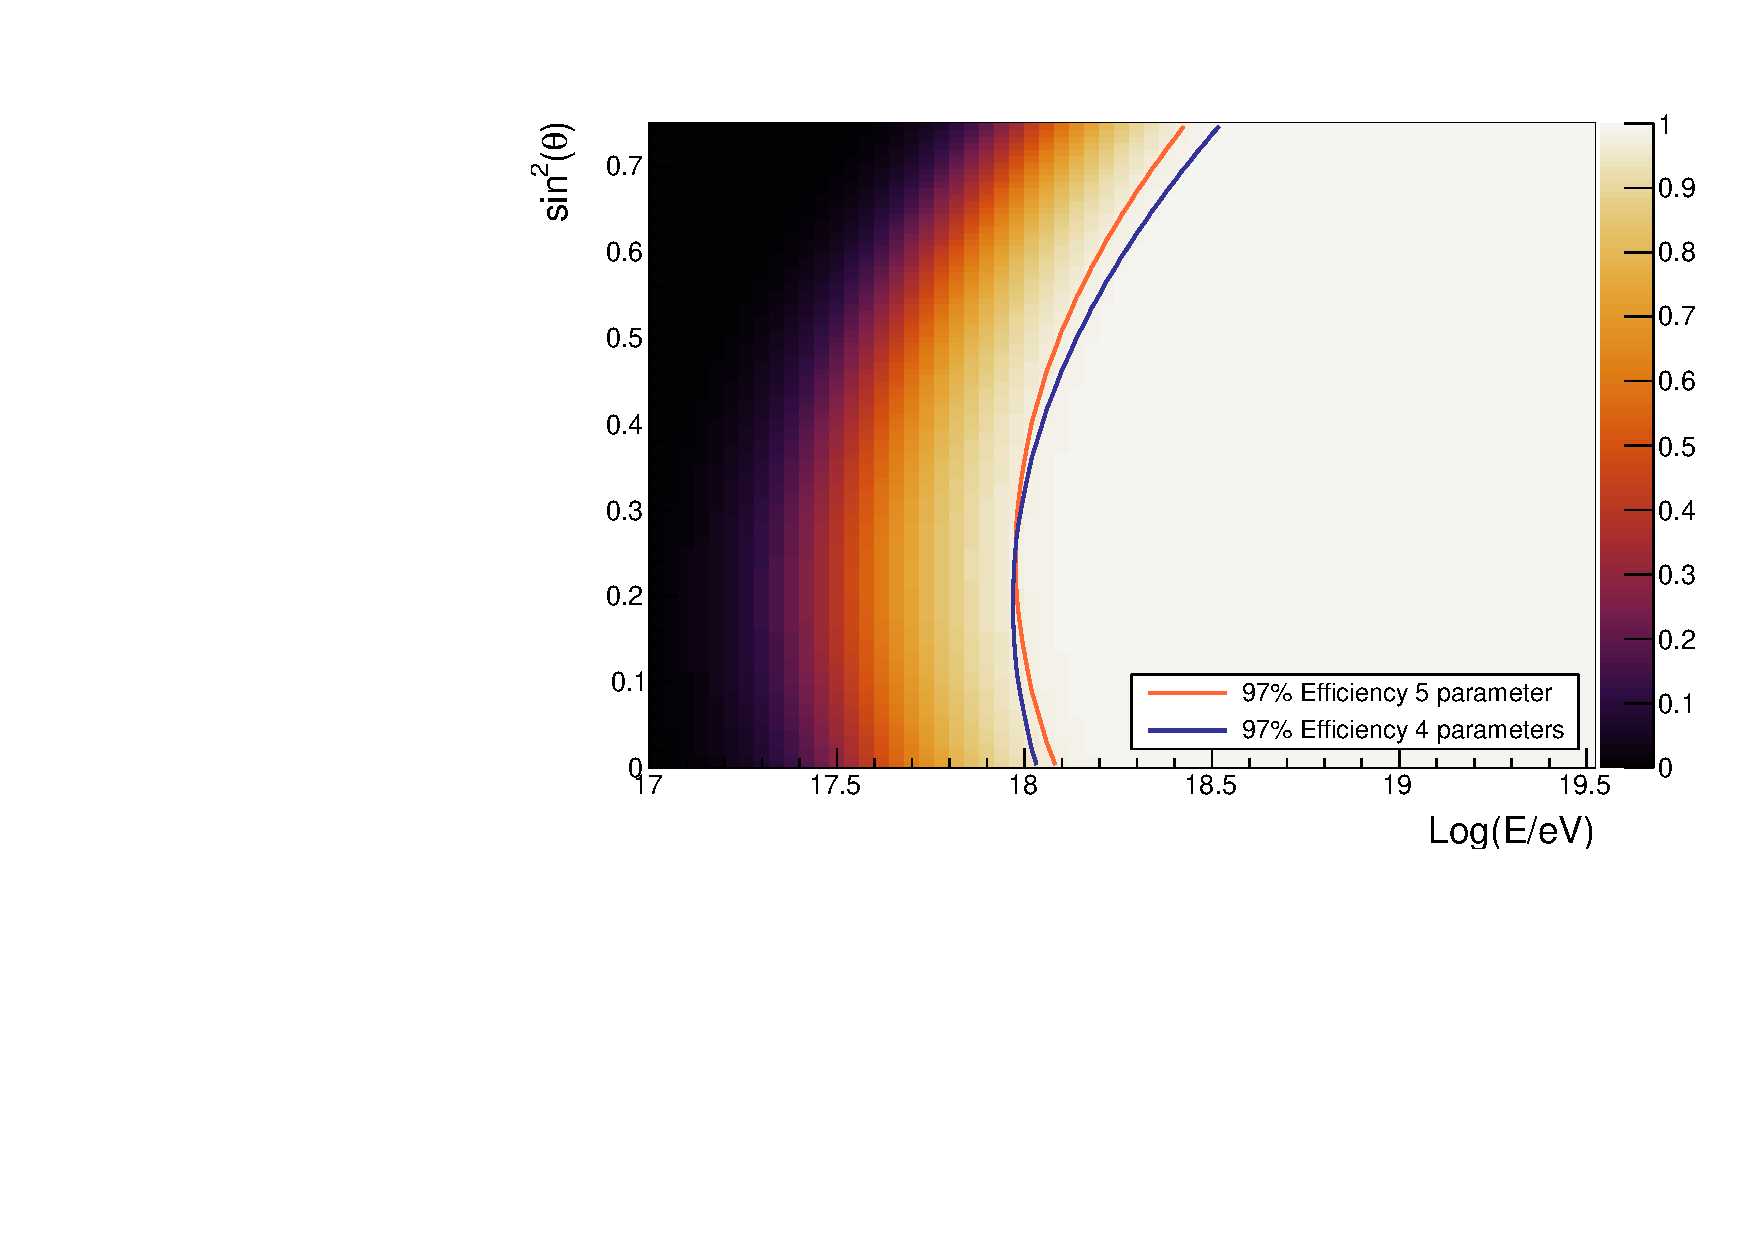
\includegraphics[width=0.7\textwidth]{plots/SurfaceNew.pdf}
        \caption{Energy and zenith angle 5 parameter fit of the SD1500 efficiency and the $97\%$ efficiency threshold.
        \label{fig:surfaceNew}}
    \end{center}
\end{figure}


\begin{thebibliography}{99}

\end{thebibliography} 

\end{document}
